%% ----------------------------------------------------------------
%% Thesis.tex -- MAIN FILE (the one that you compile with LaTeX)
%% ----------------------------------------------------------------

% Set up the document
\documentclass[12pt,a4paper,oneside]{csedu}  % Use the "Thesis" style, based on the ECS Thesis style by Steve Gunn
\graphicspath{{Figures/}}  % Location of the graphics files (set up for graphics to be in PDF format)

% Include any extra LaTeX packages required
\usepackage{graphicx}
\usepackage[square, numbers, comma, sort&compress]{natbib}  % Use the "Natbib" style for the references in the Bibliography
\usepackage{verbatim}  % Needed for the "comment" environment to make LaTeX comments
\usepackage{vector}  % Allows "\bvec{}" and "\buvec{}" for "blackboard" style bold vectors in maths
\hypersetup{urlcolor=black, colorlinks=true}  % Colours hyperlinks in blue, but this can be distracting if there are many links.
\usepackage{amsthm}
\usepackage{array}
\usepackage{tabularx}
\usepackage{multirow}
\usepackage{fixltx2e}
\usepackage[english]{babel}
\usepackage{amsmath}
\usepackage{todonotes}
\usepackage[]{algorithm2e}
\usepackage{pgfplots}
\pgfplotsset{compat=newest}

%% ----------------------------------------------------------------
\begin{document}
\frontmatter      % Begin Roman style (i, ii, iii, iv...) page numbering

% Set up the Title Page
\title{An Efficient Approach for Mining Frequent Pattern over Uncertain Data Stream}
\authors  %{\texorpdfstring
         %{\href{your website or email address}{Name}}
{Md. Badi-Uz-Zaman Shajib  \\Exam Roll: Curzon Hall-- 1089\\Registration No: EK - 899}
%{Your name should not appear on the external copies, write name between braces on the left}


%      {Author Name}
%   }
%\addresses  {\groupname\\\deptname\\\univname\\\FACULTY}  % Do not change this here, instead these must be set in the "Thesis.cls" file, please look through it instead, add roll, session and registration number ehich starts at line 204.
%\date       {\today}
%\subject    {}
%\keywords   {}

\maketitle

%% ----------------------------------------------------------------

\setstretch{1.5}  % It is better to have smaller font and larger line spacing than the other way round

% Define the page headers using the FancyHdr package and set up for one-sided printing
\fancyhead{}  % Clears all page headers and footers
\rhead{\thepage}  % Sets the right side header to show the page number
\lhead{}  % Clears the left side page header

\pagestyle{fancy}  % Finally, use the "fancy" page style to implement the FancyHdr headers

%% ----------------------------------------------------------------
% Declaration Page required for the Thesis, your institution may give you a different text to place here
\Declaration{

\addtocontents{toc}{\vspace{1em}}  % Add a gap in the Contents, for aesthetics
I declare that this thesis titled, \emph{"An Efficient Approach for Mining Frequent Pattern over Uncertain Data Stream"} and the work presented in it are my own. This work was done wholly or mainly while in candidature for a research degree at this University. Where any part of this thesis has previously been submitted for a degree or any other qualification at this University or any other institution, this has been clearly stated. Where I have consulted the published work of others, this is always clearly attributed. Where I have quoted from the work of others, the source is always given. With the exception of such quotations, this thesis is entirely my own work. I have acknowledged all main sources of help. Where the thesis is based on work done by myself jointly with others, I have made clear exactly what was done by others and what I have contributed myself.

\bigskip
\bigskip
\bigskip
\bigskip
\bigskip
\bigskip


%\begin{tabular}{lp{1in}r}
%\\ & \\ & \\


\begin{tabular}{c c c c}

  % after \\: \hline or \cline{col1-col2} \cline{col3-col4} ...
  Countersigned &\hspace{.50in} & & Signature \\

   & & &  \\
  \ldots\ldots\ldots\ldots \ldots\ldots\ldots\ldots   & & & \ldots\ldots\ldots\ldots \ldots\ldots\ldots\ldots   \\
  (Mohammad Samiullah, Lecturer) & & & (Md. Badi-Uz-Zaman Shajib) \\
  {\bf Supervisor} & & &  \\

 

\end{tabular}
}

\clearpage  % Declaration ended, now start a new page



% The Abstract Page
\addtotoc{Abstract}  % Add the "Abstract" page entry to the Contents
\abstract{
Knowledge is power. In modern times, knowledge discovery in big data is one of the most recent, interesting and popular topic for researchers. In this topic, frequent patterns finding in the large database is one of the first and important challenges. With the rapid growth of modern technology like internet, smart devices (e.g. smart phones, smart watch, smart car etc.) huge data is flowing each and every microsecond. Moreover, the incoming stream of data is not always accurate and precise. Properties of data stream flow changing each and every time with the change of interest of people that is making data dynamic. These uncertain stream data (e.g. GPS data, satellite monitoring, biometric data etc.) are the resources to many emerging applications in medical science, disaster management, national security etc. These situations increase the difficulties of extracting valuable and interesting knowledge discovery from big data. Many approaches have been developed to finding frequent patterns from uncertain data. Some have been adopted to find frequent patterns from the stream of uncertain data. Due to the uncertainty and dynamic properties of data, it becomes a great challenge to find the appropriate and efficient approach that saves resource (CPU/memory). Some approach has been developed with exact calculation and some others with the probabilistic approach. But all of them suffer from either optimization (minimum resource use) or correctness (wrong data in the result set). Moreover, most of them cannot handle the stream of data that is dynamic databases. In this thesis, we proposed an efficient, correct, optimized approach for handling uncertain data stream. We have developed a probabilistic, sliding window based approach to creating complete new \emph{US-tree} that is memory efficient and optimized. This \emph{US-tree} will keep most recent meta-information \emph{U\textsuperscript{cap}} value for further mining. A comprehensive performance analysis shows that our approach scalable, correct and faster.
\addtocontents{toc}{\vspace{1em}}  % Add a gap in the Contents, for aesthetics

 }

\clearpage  % Abstract ended, start a new page
%% ----------------------------------------------------------------

\setstretch{1.3}  % Reset the line-spacing to 1.3 for body text (if it has changed)

% The Acknowledgements page, for thanking everyone
\acknowledgements{
\addtocontents{toc}{\vspace{.5em}}  % Add a gap in the Contents, for aesthetics

First of all, I am thankful and expressing my gratefulness to Almighty Allah who offers me His divine blessings, patient, mental and psychical strength to complete this project work. I am deeply indebted to my project supervisor Mohammad Samiullah, Lecturer, Department of Computer Science and Engineering, University of Dhaka. His scholarly guidance, important suggestions, endless patience, constant supervision, valuable criticism, and enormous amount of work for going through my drafts and correcting them, and generating courage from the beginning to the end of the research work has made the completion of the project possible.\\\\
I would like to express my deep gratitude to Dr. Chowdhury Farhan Ahmed, Associate Professor, Department of Computer Science and Engineering, for his support and help for my work with his suggestions and time. The discussions with him on various topics related my works have helped me to enrich my knowledge and conception regarding this work.\\\\
Last but not the least; I am highly grateful to my parents, my wife, sisters, family members and friends for their support and constant encouragement, which have always been a source of great inspiration for me.
}
\clearpage  % End of the Acknowledgements
%% ----------------------------------------------------------------

\pagestyle{fancy}  %The page style headers have been "empty" all this time, now use the "fancy" headers as defined before to bring them back


%% ----------------------------------------------------------------
\lhead{\emph{Contents}}  % Set the left side page header to "Contents"
\tableofcontents  % Write out the Table of Contents

%% ----------------------------------------------------------------
\lhead{\emph{List of Figures}}  % Set the left side page header to "List if Figures"
\listoffigures  % Write out the List of Figures

%% ----------------------------------------------------------------
\lhead{\emph{List of Tables}}  % Set the left side page header to "List of Tables"
\listoftables  % Write out the List of Tables

%% ----------------------------------------------------------------
\addtotoc{List of Algorithms}
\lhead{List of Algorithms}  % Set the left side page header to "List of Algorithms"
\listofalgorithms
%% ----------------------------------------------------------------
\setstretch{1.5}  % Set the line spacing to 1.5, this makes the following tables easier to read
\clearpage  % Start a new page
%\lhead{\emph{Abbreviations}}  % Set the left side page header to "Abbreviations"
%\listofsymbols{ll}  % Include a list of Abbreviations (a table of two columns)
%{
% \textbf{Acronym} & \textbf{W}hat (it) \textbf{S}tands \textbf{F}or \\
%\textbf{LAH} & \textbf{L}ist \textbf{A}bbreviations \textbf{H}ere \\

%\textbf{} & \textbf{} \textbf{} \textbf{} \\
%}

%% ----------------------------------------------------------------
\clearpage  % Start a new page


\setstretch{1.5}  % Return the line spacing back to 1.3

\pagestyle{empty}  % Page style needs to be empty for this page
%\dedicatory{For/Dedicated to/To my\ldots}

\addtocontents{toc}{\vspace{2em}}  % Add a gap in the Contents, for aesthetics


%% ----------------------------------------------------------------
\mainmatter   % Begin normal, numeric (1,2,3...) page numbering
\pagestyle{fancy}  % Return the page headers back to the "fancy" style

% Include the chapters of the thesis, as separate files
% Just uncomment the lines as you write the chapters

%\documentclass{book}
%\begin{document}
\chapter{Intorduction}
\section{Mining Frequent Data}
\section{Our Contribution}
Our key contributions are given below
\begin{itemize}
\item We have introduced an prefix value for each items in a transaction which always maintain upper bound of probability. That helps us to make compact pattern tree construction.
\item A new approach \emph{US-tree} that is very much compact and very memory effecient
\item A new mining algorithm \emph{USFP-growth} that is very efficient and reduce mining time surprisingly.
\item 
\end{itemize}
\section{Thesis Organization}
We have carried out the thesis work to consummate the objectives. An outline of rest of the chapters is provided as follows:
\paragraph{Chapter 2}
Describes the necessary background study and existing approaches.
\paragraph{Chapter 3}
Provides the details of our proposed approach with required analysis.
\paragraph{Chapter 4}
Presents the results of experimental results in detail with comparison and analysis.
\paragraph{Chapter 5}
Shows several real life applications for our proposed approach and ends the thesis with a brief conclusion and future scopes.
%\end{document} % Introduction
%%
%\documentclass[a4paper,12pt]{book}
%\usepackage{fixltx2e}
%\usepackage{graphicx}	
%\begin{document}
\chapter{Background Study and Related Works}
\lhead{Chapter 2. \emph{Background Study and Related Works}}

In this chapter we have described some related work and provide some background stuffs that are  appropriate to the remainder of this paper. We have discussed about different terminology and related analysis for better understanding. We have focused the recent research works on uncertain and stream database. We have provided the analysis of existing algorithms, approaches their philosophy, working procedure, complexity analysis, aim and limitations that will help very much for better understanding and improvement of existing approaches.

\section{Data Mining}
In the previous chapter, Chapter 1 Introduction, we have described about data mining, frequent pattern mining, frequent pattern mining from uncertain data, frequent pattern mining from stream data. First one is candidate generation and test based approach named Apriori ~\cite{apriori}. Second one is pattern growth approach named as FP-growth ~\cite{fp_growth}. Apriori ~\cite{apriori} is a prior knowledge based  algorithm, that is , if any pattern is not frequent then one of its super-pattern must not be frequent.It works in a level wise approach. From the given database in each level it's generate frequent sub-patterns and merges them to propagate the candidates for next level. In this approach multiple times scan of database is mandatory and, a lot of test cases needed to be tested and for each check it is mandatory to search the database again and again. On the other hand FP-growth ~\cite{fp_growth} has been adopted divide and conquer approach. This has solved multiple scans and also reduced the huge candidate test. In this approach, firstly the huge database is compressed and put into a data structure named FP-tree holding the  itemset association information and divide such a compressed database into a set of condition databases, each associated with one frequent item, and mine the constructed conditional database recursively. Here, there is no need to generate candidate for next level or no need to generate candidate. Apriori suffers from huge candidate generation whereas FP-growth has resolved this problem. However, Apriori ~\cite{apriori} suffers much more when support factor. Thus all the approaches derived or influenced by Apriori ~\cite{apriori} (e.g U-priori ~\cite{u_priori}) also suffers form this problem.

\section{Uncertain Stream Data}
Data uncertainty is an inherent property in various applications due to reasons such as hardware fault, uncertainty of incidents, outdated sources or imprecise/incorrect measurement. In the age of Big data, uncertainty is one of the defining characteristics of data. Data is constantly growing in volume, variety, velocity and uncertainty. In a large range of applications domains uncertain data is found in abundance.  Today on the world wide web, data from sensor networks like GPS, weather ditection machines, within enterprises both in their structured and unstructured sources, biological data, meteorological trends, of medical behavior of living organisms data, human behavior, are the example of uncertain data. Customer name of a super shop is an real life example of uncertain data. For example there exists several customers named Mrs./Mr X registered in a super shop but if we want a particular Mrs./Mr. X then we will not certainly be able to find her/him by name.\\ \\
In modern age there are much more instruments we are being used to like smart-phones, smart-gears (e.g. smart watch, smart glass). All the devices has many more sensors those are collecting data each and every micro second. But all the data from the souces are imprecise/incorrect. For example a temperature sensor gives some information like current temperature is 40 degree, with \%5-10\% error. This makes this data imprecise and uncertain. Moreover, features like weather forecast is inherently uncertain. For example , todays weather forecast may be rainy but it has only 65\% confidence. There are many cases when information acquired from human experiences are not reliable and precise. Different people can describe same incident in different view and perspective. As an example, in a bird viewing event Mr. C saw a crow flying by. But, Mr. D thinks it was a raven. So, uncertainty values can be attached with these observations like the bird has 75\% probabilty to be crow and 20\% probability to be a raven.
%\documentclass{article} 
%\usepackage{graphicx}  
%\usepackage{multirow}
%\usepackage[table]{xcolor}
%\usepackage{fixltx2e}
%\usepackage{array}
%
%\begin{document}
\begin{table}[ht]
\centering

\begin{tabular}{|l|l|l|l|l|}
\hline
No & \multicolumn{4}{c|}{Items in Transaction} \\ \hline \hline
	T-1 & a(0.9) & c(0.6) & d(0.5) & e(0.2)\\\hline
	T-2 & a(0.9) & b(0.4) & e(0.1) & --    \\\hline
	T-3 & a(0.2) & c(0.9) & d(0.7) & --    \\\hline
	T-4 & b(0.3) & c(0.9) & -- & --\\\hline
	T-5 & a(0.1) & b(0.3) & c(0.9) & --    \\\hline
	T-6 & a(0.9) & e(0.3) & -- & --        \\\hline
   	T-7 & a(0.1) & d(0.6) & e(0.2) & --    \\\hline
	T-8 & a(0.1) & c(0.2) & f(0.6) & --    \\\hline
	T-9 & c(0.2) & d(0.9) & f(0.6) & --    \\\hline

	T-7 &  --  &  --  &  --  & --    \\\hline
	T-8 &  --  &  --  &  --  & --    \\\hline
	T-9 &  --  &  --  &  --  & --    \\\hline
\end{tabular}
\label{tab:ex_u}
\caption{Uncertain Stream Transaction Table}

\end{table}
%\end{document}
\subsection{Categorization of Uncertain Data}
By type of uncertainty assignment uncertain data can be categorized into three types. They are:
\paragraph{Attribute Uncertainty}
In attribute uncertainty, each uncertain attribute in a tuple has its own independent probability distribution. For example, if readings are taken of temperature and wind speed, each would be described by its own probability distribution for correctness and precision, as knowing the reading for one measurement would not provide any information about the other.
\paragraph{Correlated Uncertainty}
In correlated uncertainty, multiple attributes may be described by a joint probability distribution. For example, if there rain occurs then an musical festival event will be stopped. Then the occurrence of event depends on probability of rain. And thus this makes a co-relation with rain and musical festival
\paragraph{Tuple Uncertainty}
In tuple uncertainty, all the attributes of a tuple are subject to a joint probability distribution. This covers the case of correlated uncertainty, but also includes the case where there is a probability of a tuple not belonging in the relevant relation, which is indicated by all the probabilities not summing to one. For example, assume we have a tuple T\textsubscript{i} = \emph{(a, 0.4) | (b, 0.5)} and the probability this tuple exists in the data base is 10\%. Then this is called tuple uncertain.
		\begin{figure}
		\centering
			\includegraphics[width=1\textwidth]{../images/d_probability}
		\caption{Discrete Probability Distribution}
		\label{figure:d_probability}
		\end{figure}
		\begin{figure}
		\centering
			\includegraphics[width=1\textwidth]{../images/c_probability}
		\caption{Continuous Probability Distribution}
		\label{figure:c_probability}
		\end{figure}
\subsection{Uncertainty Types}
Uncertainty can be of two types: discrete and continuous. In this uncertainty  the probability of an uncertainty is discrete value (figure \ref{figure:d_probability}). Continuous uncertainty means the probability of an item/event being certain lies between a certain value (eg. 0 and 1) (figure \ref{figure:c_probability}). In many real-life applications, uncertain objects are already given by discrete observations, in particular if the objects are derived from sensor signals. This type of representation is motivated by the fact, in many cases, only discrete but ambiguous object information as usually returned by common sensor devices is available, e.g., discrete snapshots of continuously moving objects.

\subsection{Expected Support for Uncertain Data}
For uncertain data expected support calculation is not streight forward. The support calculation follows the following equation.
	\begin{equation}
	\emph ExpSup \qquad = \qquad \sum_{i = 0}^{UDB} [\prod_{x \in I } p(x , t_i)]
	\end{equation}
\emph {where,}	\textbf{\emph {I}} is itemset,	\textbf{\emph { p(x, ti)}} is existential probability value for any item \textbf{\emph {x}} in transaction \textbf{\emph {t\textsubscript{i}}} 	\textbf{\emph {UDB}} is an uncertain database.\\
For example let table \ref{table:uncertain_stream_transaction} be consider a uncertain database. Here expected support of itemset \emph{ab} will be $0+0.9*0.4+0+0+0.3*0.1+0+0+0+0=0.39$.

\subsection{Stream Data}
Stream data is data unbounded and continuous data incoming from any data sources that is producing all time a lots of data. These data is that much continuous and extreme in volume that storing this much data in any storage can not be thought. This much data processing and storing makes a huge cost that can be think. This stream of data is valueless unless this is processed, categorized and extract important knowledge. But this garbage can be diamond if this data is categorized and extract important information. Here data mining plays an important role.\\ \\
 For example day by day with enormous increase of internet availability and use the data producing each day by each user in every micro second is extremely huge. These big data computation is much more difficult. Particularly we can look at an example: as the social media is being popular day by day people are using these media like Facebook ~\cite{facebook}, Twitter \cite{twitter} etc. They are being used to these medias. Passing much more times and this gives a great opportunity to get a very much valuable information regarding their likes, their daily routine, their current status, their friends and families. This gives much more opportunity to profile people, categorized them. This gives the service selling organizations a great scope to digital online marketing, advertising their products and offer many promotional offers to people. Again, as this is used to communicate with each other then any terrorist activity can be predict earlier from these resources found from web. But the main difficulty is to extract information to categorized and profile these extreme data incoming from source.

\section{Existing Approaches}
Many algorithms has been developed to mine frequent itemsets from uncertain databases. Among them some are Apriori ~\cite{apriori} like approach and others are FP-growth ~\cite{fp_growth} like approach. U-Apriori ~\cite{u_priori} was proposed to mine uncertain frequent pattern that is Apriori like candidate generation and test based approach. UF-growth ~\cite{uf_growth}, UFP-growth ~\cite{ufp_growth} was proposed to mine frequent patterns from uncertain data but this suffers much more for compactness of tree. CUF-growth ~\cite{cuf_growth}, CUF-growth\textsuperscript{*} ~\cite{cuf_growth}, PUF-growth ~\cite{cuf_growth} was proposed later for mining uncertain data but they produce false positives as they works with probabilistic uncertainty modeling. All of them are unable to mine stream of uncertain data. UF-stream ~\cite{suf_growth} and SUF-growth ~\cite{suf_growth} proposed to mine uncertain frequent pattern from stream. UF-stream ~\cite{suf_growth} suffers from both false positives and false negatives. The SUF-growth ~\cite{suf_growth} is an exact mining algorithm that has resolved the false positive and false negative genration but the constructed tree structure is like UF-growth ~\cite{uf_growth} that suffers much because the data structure (tree ) SUF-growth ~\cite{suf_growth} use to keep information is not compact. Before elaborate discussion of SUF-growth ~\cite{suf_growth} we will provide a brief discussion on background of uncertain stream mining approaches.

	
	\subsection{APriori}
	Apriori ~\cite{apriori} is one of the common algorithm for data mining. It works in a level wise approach based on a prior knowledge. In each level Apriori algorithm generates frequent sub-patterns from the given database and merges them to generate the candidates for next level. That's why this kinds of algorithms called candidates generating algorithm.  Apriori is designed to operate on databases containing transactions (for example, collections of items bought by customers, or details of a website frequentation). Generating frequent sub-patterns it can use large itemset property. The sub-patterns are easily parallelized and it's easy to implement. For those reasons from it's proposed time Apriori is of the frequent used algorithm for data mining.	But, some of it's draw back many other algorithms took place over it. The draw back are given below.In APriori, number of database scan increases with the dimension of the candidate itemset.It needs transaction databases in memory resident for assumed performance. Performance suffers much in candidate set generation and test. This approach fit for frequent pattern finding from certain data but not for uncertain or stream data.
	
	\subsection{FP growth }
	FP-growth ~\cite{fp_growth} is a tree based approach that keeps meta data information in a compressed tree structure. It named the tree structure is FP-tree. In this tree node share is possible. So the data structure becomes very compressed. It can store much more data of the transaction database. Later mining algorithm is used to extract frequet patterns. This has solved the candidate generation of Apriori ~\cite{apriori} algorithm and also the huge test. Fp-growth mining algorithm use divide and conquer approach for candidate frequent sub-pattern mining. It first generates the candidate sub-pattern tree and then mine recursively. This is one of the very first idea of frequent pattern mining. This approach also designed for certain data and does not fit for data stream.
	
	\subsection{U-Priori}
	U-Apriori ~\cite{u_priori} is a  modification of Apriori ~\cite{apriori} algorithm which is proposed to handle uncertain data. We already know in Apriori ~\cite{apriori} algorithm support count play an important role. Number of databases scan and candidate for next level depends on support count. The modification of Apriori in U-Apriori is support count. It has designed for handling support using minimum support calculation of uncertain data. Specially, instead of incrementing the support counts of candidate patterns by their actual support, U-Apriori increments the support countsof candidate patterns by their given support count using the uncertain support count equation. Though U-Apriori come over Apriori to solve support count problem of uncertain data but U-Apriori suffers from the some problems. As U-Apriori is a modification of the Apriori algorithm, performance of U-Apriori algorithm for large scale of data because it follows level wise sub-patterns generation and merge to generate candidate for next level. That's why number of databases scan increase with the dimension of itemset. If the existential probabilities of most items within a pattern I are small, increments for each transaction can be insignificantly small. Consequently, many candidates would not be recognized as infrequent until most transaction were processed.  
	
	\subsection{UF-growth}
	Observing outperforms of FP-growth ~\cite{fp_growth} over Apriori ~\cite{apriori}, UF-growth ~\cite{uf_growth} was proposed for mining uncertain data. We know key to success of FP-growth over Apriori is FP-tree, which is a compact tree structure capturing frequent items within transactions in the databases of precise data. Like FP-growth, UF-growth also used the tree construction approach. This constructs UF-tree By extracting appropriate tree paths to construct subsequent FP-trees, frequent itemset can be mined. Each tree path represents a transaction. Each node in a tree path captures(i) an item x and (ii) its actual support(i.e, occurrence count of x in that tree path). Tree paths (from the root) are merged if they share the same items(i.e., the captured tow items share a node if they has both same item id and same existential probability). Due to this path sharing, the UF-tree is usually compact. However, as dealing with uncertain data, the situation is different form certain data. The expected support of any itemset X is the sum of products of existential probability of items within X. Hence, UF-growth uses a UF-tree to capture frequent items within transactions of uncertain data. Each node in an UF-tree captures (i) an item x, (ii) its existential probability value, and (iii) the occurrence count of x in that tree path. By doing so, UF-growth finds all and only those frequent itemsets by computing the expected support of an itemset X (as the sum of products of the captured existential probability values). Tree paths are merged if they share the same items and existential probability values. Consequently, UF-trees may not be as compact as FP-trees. In real life scenirio this tree is never compact. And mining suffers much more as the candidate for sub-pattern tree grows as the transaction grows.
	
	\subsection{UFP-growth}
	To reduce the tree size in UF-tree of UF-growth ~\cite{uf_growth}, UFP-growth ~\cite{ufp_growth} was proposed. In this approach, items are grouped and share same node (i.e., nodes with the same x but similar existential probability values) into a cluster. Each cluster of the item x captures (i) the maximum existential probability value of all nodes within the cluster and (ii) the number of existential probability values in each cluster. Depending on the clustering parameter, the resulting tree namely, UFP-tree may be as large as the UF-tree (i.e., no reduction in tree size). On the other hand, if the UFP-tree  is smaller than the UF-tree, then UFP-growth may return approximate results (e.g., with false positives or infrequent itemsets). Though it solves some tree compactness problem but the tree is still not that much compact. More over this do not fit for uncertain stream data. 
	
	\subsection{PUF-growth}
	To reduce the size of the UF-tree ~\cite{uf_growth} and UFP-tree ~\cite{ufp_growth}, the prefix-capped uncertain frequent pattern tree, PUF-tree structure and mining algorithm PUF-growth ~\cite{puf_growth} was proposed, in which important information about uncertain data is captured so that frequent patterns can be mined from the tree. The PUF-tree  is constructed by considering an upper bound of existential probability value for each item  which is named as I\textsuperscript{cap}. When generating a k-itemset (where $k>1$). This upper bound of an item x\textsubscript{r} in a transaction t\textsubscript{j} is called the (prefixed) item cap, I\textsuperscript{cap} of x\textsubscript{r} in t\textsubscript{j}. Thus PUF-tree is very much compact. This approach generates some false positive. But the false positive reduction technique makes this a stronger approch. But this is not fit for uncertain stream data. 
	
	\subsection{UF-streaming}
	UF-streaming ~\cite{suf_growth} was proposed to mine frequent item from uncertain stream data. This is a window and batch based approach that capture most recent data, as most recent data is most important. It has divided the transaction streamd data in several batch each batch is inserted into tree structure that is UF-tree ~\cite{uf_growth} and mine each tree using UF-growth ~\cite{uf_growth} and put all the frequent patterns found in a UF-stream structure. For avoiding false negative they have used a value preMinSup less then mininum support (0 < preMinSup < minimum support). Then untill window is completed the frequent itemset is put into UF-stream tree structure. This has addressed the problems of stream uncertain data mining but it suffers from some problems given below.
	\begin{itemize}
		\item Un-necessary mining each batch. Let window size is 3 and batch size is 2. If one wants the mining result at window 50 then in this approach it is needed to mine each of 1 to 50 batch for getting the result.
		\item The used tree structure is UF-tree that suffers from compactness problem.
		\item Extra data structure for keeping frequent itemset UF-stream tree structure.
		\item False positive generation in the mining process.
		\item False negative generation in the mining process.
		\item This has high running time and memory consumption.
	\end{itemize}
	
	\subsection{SUF-growth}
	SUF-growth ~\cite{suf_growth} addressed the limitations exist in UF-streaming ~\cite{suf_growth}. SUF-growth algorithm outperforms over UF-streaming algorithm. It improves over UF-streaming by avoiding the aforementioned potential problems for mining frequent itemset from streams of uncertain data. SUF-growth is an exact algorithm. Its means SUF-growth returns only truly frequent itemset. Where UF-streaming returns both true or false frequent itemset. Its use only minsup. No need to use preMinsup. There also have any problem of finding an appropriate value of preMinsup. This algorithm does not need UF-stream structure to store the mined itemsets. Need transaction databases in memory resident for assumed performance. Instead of this its use delayed mode for mining. As a result unnecessary computation could be reduced and unnecessary mining is avoided.
		\begin{figure}[]
		\centering
			\includegraphics[width=1\textwidth]{../images/suf_simulation}
		\caption{SUF-growth ~\cite{suf_growth} tree construction}
		\label{figure:suf_simulation}
		\end{figure}
	Considering the advantages of SUF-growth over others algorithm there is question. The is how SUF-growth ~\cite{suf_growth} algorithm find frequent itemsets from streams of uncertain data using a new tree structure called SUF-tree. Now we describe about this. We first construct a SUF-tree, and then extract relevant paths from this SUF-tree (which is a global tree) to recursively form smaller UF-trees for projected databases. Due to the dynamic nature and Property 2 of data streams, expected support of items is continuously affected by the arrival of new batches (and the removal of the contents of older batches). Arranging items in frequency-dependent order in the SUF-tree may lead to swapping—which, in turn, can cause merging and splitting—of tree nodes when the global frequencies of items change. Hence, in the SUF-tree, items are arranged according to some canonical order (e.g., lexicographic order), which can be specified by the user prior to the construction of the SUF-tree or the mining process. Consequently, the SUF-tree can be constructed using only one scan of the streams of uncertain data, and the resulting SUF-tree captures the contents of the streams. Moreover, the SUF-tree preserves the usual tree properties. The occurrence count of a node is at least as high as the sum of occurrence counts of its children.The ordering of items is unaffected by the continuous changes in the expected support values of items.\\ \\
	For example for table \ref{table:uncertain_stream_transaction} transaction database let construct the SUF-tree. Figure \ref{figure:suf_simulation} shows the construction of the SUF-tree. Here as the suff tree is based on UF-tree construction approach the node sharing is very rare. From figure \ref{figure:suf_simulation} its clearly visiable that the node sharing is not that much impressive as the node should be shared if the two same item has same existential probability and in real life scenirio this sharing is very rare. For this reason \emph{a(0.9)} in \emph{T\textsubscript{1}} and \emph{a(0.2)} in \emph{T\textsubscript{3}} did not share single node and the tree compactness could not be accomplished.
	Although the SUF-growth has resolved some limitations of UF-streaming ~\cite{suf_growth}, some limitations still exists. The findings are listed below:
	\begin{itemize}
		\item The tree structure it uses is UF-tree ~\cite{uf_growth} structure which suffers from compactness. So SUF-growth tree also inherit this limitation.
		\item The tree construction cost will be much more (both running time and memory) as the transaction grows.
		\item The mining algorithm it uses is FP-groth like approach that generates a huge candidate sub-pattern tree that costs much in the mining time. It increase mining cost (both running time and memory).
 	\end{itemize}
	
\section{Summary}
The approaches for finding frequent patterns on uncertain data is challanging because of data uncertainty property. Althogh many of the approaches has been adopted to address and solve this constrains but still there are limitations. Moreover there is still limitations in mining uncertain stream. The compressed data structure designe is a tough challange for uncertain stream data. Later chapters we will provide a novel, completely new and effecient data structure that will make the tree compactness more and gain both running time and memory efficiency.
%\end{document} % Previous Work
%%%
\documentclass[a4paper,12pt]{book}
\usepackage[english]{babel}	
\usepackage[nottoc]{tocbibind}
\usepackage{graphicx}  
\usepackage{multirow}
\usepackage{xcolor}
\usepackage{fixltx2e}
\usepackage{caption}
\usepackage{subcaption}
\usepackage{array}
\usepackage[english]{babel}
\usepackage[utf8]{inputenc}
\usepackage{amsmath}
\usepackage{amsfonts}
\usepackage{graphicx}
\usepackage{todonotes}
\usepackage[]{algorithm2e}

\begin{document}
\chapter{Our Proposed Approaches}
\input{pa_intro}
\section{Uncertain Stream Data Properties}
In this chapter we will talk about data properties. our data has two special properties. (1)Stream and (2)Uncertainty. For these properties it becomes very much hard to get valuable and interesting information from data. So first we discuss about the data set properties.
%\documentclass{article} 
%\usepackage{graphicx}  
%\usepackage{multirow}
%\usepackage[table]{xcolor}
%\usepackage{fixltx2e}
%\usepackage{array}
%
%\begin{document}
\begin{table}[ht]
\centering

\begin{tabular}{|l|l|l|l|l|}
\hline
No & \multicolumn{4}{c|}{Items in Transaction} \\ \hline \hline
	T-1 & a(0.9) & c(0.6) & d(0.5) & e(0.2)\\\hline
	T-2 & a(0.9) & b(0.4) & e(0.1) & --    \\\hline
	T-3 & a(0.2) & c(0.9) & d(0.7) & --    \\\hline
	T-4 & b(0.3) & c(0.9) & -- & --\\\hline
	T-5 & a(0.1) & b(0.3) & c(0.9) & --    \\\hline
	T-6 & a(0.9) & e(0.3) & -- & --        \\\hline
   	T-7 & a(0.1) & d(0.6) & e(0.2) & --    \\\hline
	T-8 & a(0.1) & c(0.2) & f(0.6) & --    \\\hline
	T-9 & c(0.2) & d(0.9) & f(0.6) & --    \\\hline

	T-7 &  --  &  --  &  --  & --    \\\hline
	T-8 &  --  &  --  &  --  & --    \\\hline
	T-9 &  --  &  --  &  --  & --    \\\hline
\end{tabular}
\label{tab:ex_u}
\caption{Uncertain Stream Transaction Table}

\end{table}
%\end{document}
\subsection{Stream Property}
Stream data are such data those come and go away. They can not be stored in any patterns. Data streams are continuous and unbounded. This property makes finding patterns so much difficult. As when stream flows away we lose them, we have no choice to store data and scan more than one time we have to find some technique to store valuable information that will help to find valuable information later. For example table-\ref{table:uncertain_stream_transaction} shows the stream transaction database. Here \emph{T\textsubscript{1}, T\textsubscript{2}, T\textsubscript{3}, T\textsubscript{4}, T\textsubscript{5}, T\textsubscript{6}, T\textsubscript{7}, T\textsubscript{8}, T\textsubscript{9}} comes one after another and goes away. It may occur that when \emph{T\textsubscript{10}} comes after a long time of \emph{T\textsubscript{4} or T\textsubscript{5} or T\textsubscript{6}} came. So there is no way get \emph{T\textsubscript{4}} when \emph{T\textsubscript{10}} comes. As we are always interested in most recent data, because most recent data are most valuable, we proposed a sliding window based approach that holds the most recent data in our proposed \emph{US-tree} to hold valuable information for further valuable information extraction.
\subsection{Uncertainty Property}
Data is not always precise. Hardware limitations, loss of information during transmission, sampling errors etc can make precise data uncertain. For this reason the data existence is not for sure. Each time data can comes with a probability value that is called its existential probability. For example in table-\ref{table:uncertain_stream_transaction}  we can see each transaction having items with item's probability. This value is its existential probability. Let for transaction-\emph{T\textsubscript{2}} there is four items \emph{a(0.9), c(0.6), d(0.5)} and \emph{e(0.2)}. Here \emph{0.9, 0.6, 0.5, 0.2} all are existential probability of corresponding \emph{a, c, d, e}. That means \emph{a's} existential probability is \emph{0.9}. Probability of existence of \emph{a} in that transaction is \emph{0.9}. This property makes mining very much difficult. This property says that in different transaction in a transaction data base same item can have different existential probability. So finding similarity between same item becomes another matter to worry about. For expected support calculation of item becomes very much tough. For expected support calculation equation-\ref{equation:exp_sup} is used.
\input{../example/eqn_exp_sup}
From this equation we can see that calculation of support is not that easy and straight forward like certain data. Certain data support is calculated just counting the total existence of that items in the transaction were as for uncertain data it depends on its existential probability. It may occur that some data set exists many times in a transaction database but with a low probability, so ultimately the data must not be frequent. For example for table-\ref{table:uncertain_stream_transaction} if we want to find the support of \emph{ae} then we need to do the following calculation. For \emph{T\textsubscript{2}} $0.9*0.2=0.18$, \emph{T\textsubscript{2}} $0.9*0.1=0.09$, \emph{T\textsubscript{3}} $0.0$, \emph{T\textsubscript{4}} $0.0$, \emph{T\textsubscript{5}} $0.0$, \emph{T\textsubscript{6}} $0.9*0.3=0.27$, \emph{T\textsubscript{7}} $0.1*0.2=0.02$, \emph{T\textsubscript{8}}=$0.0$ and \emph{T\textsubscript{9}}=$0.0$.\\$Sup_{ae}\\=Sup_{ae(T_1)}+Sup_{ae(T_2)}+Sup_{ae(T_3)}+Sup_{ae(T_4)}+Sup_{ae(T_5)}+Sup_{ae(T_6)}+Sup_{ae(T_7)}+Sup_{ae(T_8)}+Sup_{ae(T_9)}\\=0.18+0.09+0.0+0.0+0.0+0.27+0.0+0.02+0.0+0.0=0.54$\\ So if \emph{minimum support is $0.9$} than \emph{ae} is not frequent but \emph{ae} exists four times in the transaction. So it makes very much difficult to find which is important pattern and which is not.
\newpage
\section{Preliminaries}
%\documentclass{article}
%\usepackage{fixltx2e}
%\usepackage{amsmath}
%\begin{document}
\subsection*{}
\textbf{Definition-1: Uncertain Frequent Pattern} Given DB = \emph{\{T\textsubscript{1}, T\textsubscript{2}, T\textsubscript{3} . . . T\textsubscript{N} \}} , an uncertain database with \emph{N} transactions where minimum expected support threshold is $\delta$. The problem is to mine frequent item-sets \emph{FI} $\subset$ DB, where $ExpSup(FI_i) \geq \delta $ and $FI_i \in FI$.
\subsection*{}
\textbf{Definition-2 : Batch} A group of consecutive transactions from a transaction \emph{DB}inserted in \emph{US-tree} at a time. Let table-\ref{table:uncertain_stream_transaction} batch size = \emph{3}. \emph{T\textsubscript{1}, T\textsubscript{2}, T\textsubscript{3}} is one batch and its batch-1. Then next three \emph{T\textsubscript{4}, T\textsubscript{5}, T\textsubscript{6}} is one batch and its batch-2.
\subsection*{}
\textbf{Definition-3 : Window} Window is the size of batch consecutive one \emph{US-tree} can hold. Let table-\ref{table:transaction_batch} be an example of grouped transaction and batch number tagged. So for window size \emph{2} The in a certain time batch-1 and batch-2 will create a window. then after some times when batch-3 comes then batch-2 and batch-3 will create the next window.
\subsection*{}
\textbf{Definition-4 : U\textsuperscript{cap}} The following equation is for cap calculation.
\documentclass{article}
\usepackage{amsmath}
\begin{document}
  \begin{equation}
\text{\emph{U\textsuperscript{cap}}}(X_r, t_j) =\begin{cases}
              P(X_r, t_j), & \text{if $ h > 1$}\\
              P(X_1, t_j), & \text{if $ h = 1$}
\end{cases}
\end{equation}
\end{document}
\\
For transaction \emph{DB} example in table-\ref{table:uncertain_stream_transaction} for \emph{T\textsubscript{1}}, \emph{U\textsuperscript{cap}} of \emph{a{0.9}} is $0.9$ as a is the first item. For \emph{c(0.6)} \emph{U\textsuperscript{cap}} is $0.9*0.6=0.45$, \emph{d(0.50)} \emph{U\textsuperscript{cap}} is $0.9*0.5=0.45$ and \emph{e(0.2)} \emph{U\textsuperscript{cap}} is $0.9*0.2=0.18$. \emph{U\textsuperscript{cap}} is the upper bound of existential probability. As we are taking the max of all previous items coming in a particular order all items or item sets having existential probability must be less than or equal \emph{U\textsuperscript{cap}}. that is $\forall(i,j)\{ P(I_i)*P(I_j)\leq U_{cap}(I_j)\}$ where $i < j$. So support must be less than or equal \emph{U\textsubscript{cap}}.
%
%\end{document}
\input{../example/table_uncertain_transaction_batch}
\section{Mining Frequent Patterns from Uncertain Databases}
Our proposed algorithm is divided into five parts. (1) Grouping transactions into batches and window and giving each item in a transaction a prefix value is called \emph{U\textsuperscript{cap}}. (2) insert transaction into \emph {US-tree}. (3) sliding the \emph {US-tree} (4) mining the \emph {US-tree} with \emph{USFP-growth} algorithm and (5) Eliminating false positive (not frequent but exists in frequent item set) . For simulating our approach we consider Table~\ref{table:uncertain_stream_transaction} as uncertain stream transaction data. For this simulation we consider window size as 2 and batch size 3. That means 3 transactions creates a batch and 2 batches create a window. After completing window construction (inserting batch 1 and 2) the \emph {US-tree} will be full. When new batch comes we slide the window. That means we remove oldest batch batch-1 and put batch-2 as the old batch. Then insert new batch in the tree as batch-3. So for window size 2 the tree always contains at most 2 batches. Thus the tree always holds the latest information. In next subsections we will elaborately explain our approach of every steps.
\subsection{Preparation}
\input{../example/table_prefix}
%\documentclass{article}
%\usepackage{fixltx2e}
%\begin{document}
\subsection*{}
\noindent
In this section we will describe the batch and window grouping and the prefix value \emph{U\textsuperscript{cap}} calculation. First we calculate batch and window calculation and grouping our transaction data. As we describe earlier for the example Table-\ref{table:uncertain_stream_transaction} easy simulation we take batch size as \emph{$3$} and window size as \emph{$2$}. So first \emph{$3$} transactions \emph{T\textsubscript{1}}, \emph{T\textsubscript{2}} and \emph{T\textsubscript{3}} are grouped and labeled as \emph{Batch-1}. Then next \emph{$3$} \emph{T\textsubscript{4}}, \emph{T\textsubscript{5}} and \emph{T\textsubscript{6}} are grouped together and labeled as \emph{Batch-2}. Next \emph{$3$} \emph{T\textsubscript{7}}, \emph{T\textsubscript{8}} and \emph{T\textsubscript{9}} are grouped together and labeled as \emph{Batch-3}. Thus the consecutive next \emph{$3$} transaction should be grouped as batch and ready to be inserted into \emph{US-tree}. As our window size is $2$, after inserting two batches into the \emph{US-tree} the window will be completed. Before inserting next batch \emph{Batch-3} we need to remove \emph{Batch-1}(oldest one) from tree and move \emph{Batch-2} to \emph{Batch-1 's} position and then insert new batch, \emph{Batch-3}. Thus the latest information is inserted and kept into the \emph{US-tree}. Table-\ref{table:transaction_batch} shows the window and batch grouped for stream transaction example Table-\ref{table:uncertain_stream_transaction}.

\subsection*{}
\noindent
For this calculation we earlier proposed an equation \ref{eqn_ucap}. From this equation we can create \emph{U\textsuperscript{cap}} for each item in a transaction. And thus for all transactions in the data stream. To calculate one transaction, for each item in a transaction, if item is the first item in a transaction than item's existential probability is its \emph{U\textsuperscript{cap}} value, otherwise item's \emph{U\textsuperscript{cap}} is max of previous items existential probability multiplied by item's  own existential probability. For example let Table-\ref{table:transaction_batch} T1 is \emph{a(0.9), c(0.6), d(0.5), e(0.2)}. 
In this transaction item \emph{a(0.9)} is the first item. So its \emph{U\textsuperscript{cap}} is 0.9. 
For second item, \emph{c(0.60)} previous item is only \emph{a(0.90)}. So c's $\emph{U\textsuperscript{cap}} = 0.9*0.6 = 0.54$. 
For third item, \emph{d(0.50)} there are two items before it, \emph{a(0.9)} and \emph{c(0.6)}. Among them \emph{a} has max existential probability, that is \emph{0.9}. So \emph{d's } $\emph{U\textsuperscript{cap}} = 0.9*0.5 = 0.45$. 
For fourth item \emph{e(0.2)} there are three items before it, \emph{a(0.9)} ,\emph{c(0.6)} and \emph{d(0.5)}. Among them \emph{a} has max existential probability is \emph{0.9}. So \emph{e's}  $\emph{U\textsuperscript{cap}} = 0.9*0.2 = 0.45$. Thus we can calculate each item's \emph{U\textsuperscript{cap}} value for a transaction. For easier understanding we have calculated all the item's \emph{U\textsuperscript{cap}} of Table-\ref{table:transaction_batch} and put into Table-\ref{table:prefix_assigned}.
%\end{document}
\subsection{US-tree Construction}
\paragraph*{}
\emph{U\textsuperscript{cap}}  

In this section we will describe about our tree construction \emph{US-tree}. We have describe earlier about our batch and window. A batch should be inserted into the tree in it's own window slot. After inserting all batches of to full the window, the window shall be complete and be ready to mine. We said earlier section that our tree will be very compact. For this we have proposed an approach for sharing nodes. For sharing same tree nodes two items with same id and order should not care about own existential probability. If item is already in the tree with same id then two items should share the node. Thus the tree will be very compact.When inserting an item in the tree the \emph{U\textsuperscript{cap}}  of the tree should be updated by adding the prefix value of the node. Thus each batch should be inserted into the tree. FOR EXAMPLE TABLE REF. We 
\subsection{Mining US-tree FPUS-growth}
%\documentclass{article}
%\usepackage{caption}
%\usepackage{graphicx}
%\begin{document}
\subsection*{}
In this section we will discuss about our mining algorithm \emph{USFP-growth}(algorithm-\ref{algorithm:mine}) That will find frequent patterns. For mining we used \emph{FP-growth} like approach. Generally, we can remove all the nodes having support less than \emph{minimum support}. From headr table we get such information that which nodes are less than \emph{minimum support}. We told earlier that for \emph{U\textsuperscript{cap}} value we took the upper limit, we also can we can remove all the nodes having prefix value less than \emph{minimum support}. In this process we can eliminate most of the infrequent nodes from tree. For this purpose we used header table that was created when creating the \emph{US-tree}. Then we construct conditional tree starting from the lowest support holding node. From header table we also get the position of all nodes containing same item in the tree. 
\subsection*{}
Lets mine the tree we constructed earlier. Figure-\ref{figure:min_before} is \emph{US-Tree} for mining and corresponding header table before starting mining. From the header table we get that support of \emph{a} is $3.00$, \emph{b} is $1.00$, \emph{c} is $3.30$, \emph{d} is $1.20$, \emph{e} is $0.60$. So \emph{e} is not frequent for one item set frequent pattern. So it is sure that no item set contains \emph{e} will be frequent. That is the basic upward closure property of frequent item set. So we remove all the nodes of \emph{e} and get the new mining tree Figure-\ref{figure:min_ready}. And its corresponding header. Here we find all one item sets that are frequent and that is \emph{\{a\}, \{b\}, \{c\} \{d\}} Now we will construct conditional tree for the found frequent one item and mine the conditional tree. But items having total \emph{U\textsuperscript{cap}} less than \emph{minimum support} is not needed to construct conditional tree because this \emph{U\textsuperscript{cap}} value has been take as the upper bound. So total \emph{U\textsuperscript{cap}} value less than \emph{minimum support} indicates that item must not be exists in the $2$ or more frequent item set. So we do not construct conditional tree for these items.
\subsection*{}
We construct conditional tree from items having lowest total \emph{U\textsuperscript{cap}} value greater than \emph{minimum support}. As \emph{b} having total \emph{U\textsuperscript{cap}} is $.69$ \emph{b} is ignored for constructing conditional tree. Then the next candidate is \emph{d}. From header table pointer we find that there is only one path item \emph{d} exists in the mining tree Figure-\ref{figure:min_ready}. That is \{\emph{a, c, d}\}:$1.08$. So we create conditional tree and update all nodes mining probability with \emph{d's} \emph{U\textsuperscript{cap}} $1.08$. For this conditional tree Figure-\ref{figure:d_cond} the header tables says all the nodes in the tree are having \emph{U\textsuperscript{cap}} greater than \emph{minimum support} $.9$. So all the items are ready to be constructed as conditional tree. As here is only one branch so we do not further construct conditional tree and take all the combinations as frequent items Figure-\ref{figure:d_cond} Table. so we find \emph{\{dc\}, \{da\}, \{dca\}} as frequent pattern. Next we create conditional tree for \emph{c}. Here c exists in the tree for three path those are \emph{\{a, c\} : $0.72$ , \{a , b, c\} : $.027$ and \{b, c\} : $0.27$}. So we create conditional tree (Figure-\ref{figure:c_cond}). Total mining value of \emph{c} is the sum of item caps in each respective path of \emph{c}. From the header we see that  \emph{b} has total cap having less than \emph{minimum support} so we remove \emph{b} and create two item set \emph{\{ca\}}. Next we construct \emph{ca} conditional tree that contains only root (\emph{\{\}}). So no further tree is needed to be constructed and minned. Than we create conditional tree for \emph{a}. And find only root \emph{\{\}}. Thus we get all the  frequent patterns. All the patterns are \emph{\{a\}, \{b\}, \{c\} \{d\}, \{dc\}, \{da\}, \{dca\} and \{ca\}}. As we have found all patterns from upper bound, so that it is guaranteed that there will be no false negative. But some false positive can be exists in the found frequent item set as there may be some value less than max value we assumed. so in the next section we will show an approach that eliminates the all false positives (if exists) in the data set.
%\documentclass{article}
%\usepackage{caption}
%\usepackage{graphicx}
%\begin{document}
\begin{figure}
\begin{minipage}{0.40\textwidth}
  \centering
  
	\begin{center}
	\begin{tabular}{ |c|c|c| } 
 	\hline
 		Item&\emph{U\textsuperscript{cap}}&Support\\ \hline\hline
 		A &  3.00  & 3.00\\ \hline
 		C &  1.26  & 3.30\\ \hline
 		D &  1.08  & 1.20\\ \hline
 		B &  0.69  & 1.00\\ \hline
\end{tabular}
\end{center}  
  
  
  \captionof{table}{Header Table for }
\end{minipage}
\hfill
\begin{minipage}{0.40\textwidth}
  \centering
  \includegraphics[width=\textwidth]{../images/M_TREE.jpg}
  \captionof{figure}{\emph{US-tree} Before Mining}
\end{minipage}


\caption{\emph{US-tree} and its Header Table}
\end{figure}
\begin{figure}

\begin{minipage}{0.40\textwidth}
  \centering
  
	\begin{center}
	\begin{tabular}{ |c|c|c| } 
 	\hline
 		Item&\emph{U\textsuperscript{cap}}&Support\\ \hline\hline
 		A &  3.00  & 3.00	\\ \hline
 		C &  1.26  & 3.30	\\ \hline
 		D &  1.08  & 1.20	\\ \hline
 		E &  0.54  & 0.60	\\ \hline
 		B &  0.69  & 1.00	\\ \hline
\end{tabular}
\end{center}  
  
  
  \captionof{table}{Header Table }
\end{minipage}
\hfill
\begin{minipage}{0.40\textwidth}
  \centering
  \includegraphics[width=\textwidth]{../images/sim_06.jpg}
  \captionof{figure}{\emph{US-tree} for mining.}
\end{minipage}
\caption{\emph{US-tree(Mining)} and its Header Table}
\end{figure}
%\end{document}
\documentclass{article}
\usepackage{caption}
\usepackage{graphicx}
\begin{document}
\fbox{ 
{\centering
\begin{minipage}{0.40\textwidth}
  \centering
  
	\begin{center}
	\begin{tabular}{ |c|c| } 
 	\hline
 		Item&Value\\ \hline\hline
 		a &  1.08  	\\ \hline
 		c &  1.08   	\\ \hline
 		
\end{tabular}
\end{center}  

  
  \captionof{table}{\emph{d-cond tree} Header }
\end{minipage}
  \hfill
\hfill
\begin{minipage}{0.23\textwidth}
  \centering
  \hfill
  \includegraphics[width=.8\textwidth, height=5cm]{../images/D_COND.jpg}
  \captionof{figure}{\emph{d-cond} Tree}
  \hfill
  
\end{minipage}
\hfill
\begin{minipage}{0.30\textwidth}
  \centering
  
	\begin{center}
	\begin{tabular}{ |c| } 
 	\hline
 		Freq Patterns \\ \hline\hline
 		dc  	\\ \hline
 		da   	\\ \hline
 		dca   	\\ \hline
 		
\end{tabular}
\end{center}  

  
  \captionof{table}{ \emph{Frequent Patterns for d} }
\end{minipage}
}
}

\end{document}

%\end{document}
\newpage
\subsection{False positive reduction}


\paragraph{This Is Elemininition Paragraph}
%\documentclass{article}
%\usepackage{fixltx2e}
%\usepackage{caption}
%\usepackage{graphicx}
%\begin{document}
\begin{figure}
\begin{minipage}{0.60\textwidth}
  \centering
  
	\begin{center}
	\begin{tabular}{ |c| } 
 	\hline
 		Frequent Items\\ \hline\hline
 		a \\ \hline
 		b \\ \hline
 		c \\ \hline
 		d \\ \hline
 		dc \\ \hline
 		da \\ \hline
 		dca \\ \hline
 		ca \\ \hline
\end{tabular}
\end{center}  
  
  
  \captionof{table}{\emph{Frequent Items}\\(with false positive)}
\end{minipage}
\hfill
\begin{minipage}{0.40\textwidth}
  \centering
  \includegraphics[width=\textwidth]{../images/frequent_tree.jpg}
  \captionof{figure}{\emph{Frequent Item Tree} }
\end{minipage}
\end{figure}
\begin{figure}
\begin{minipage}{.6\textwidth}
  \centering
  
	\begin{center}
	\begin{tabular}{ |c|c| } 
 	\hline
 		No & Items \\ \hline\hline
 		a  & \emph{a(0.9),c(0.6),d(0.5)}\\ \hline
 		b & \emph{a(0.9),b(0.4),e(0.1)}\\ \hline
 		c & \emph{a(0.2),c(0.9),d(0.7)}\\ \hline
 		d & \emph{b(0.3),c(0.9)}\\ \hline
 		dc& \emph{a(0.1),b(0.3),c(0.9)} \\ \hline
 		da & \emph{a(0.9),e(0.3)
}\\ \hline
\end{tabular}
\end{center}  
  
  
  \captionof{table}{Transaction Table after removing Infrequent Items}
\end{minipage}
\hfill
\begin{minipage}{0.40\textwidth}
  \centering
  \includegraphics[width=.8\textwidth]{../images/frequent_tree_final.jpg}
  \captionof{figure}{\emph{Frequent Item Tree} identifying false positives}
\end{minipage}

\end{figure}
%\end{document}


\newpage
\subsection{Algorithm}
\documentclass[a4paper]{article}

\usepackage[english]{babel}
\usepackage[utf8]{inputenc}
\usepackage{amsmath}
\usepackage{amsfonts}
\usepackage{graphicx}
\usepackage[colorinlistoftodos]{todonotes}
\usepackage{algorithm}
\usepackage{algpseudocode}
\usepackage{geometry}

\begin{document}
\paragraph*{}
Our proposed algorithm is given here.
%\documentclass{article}
%\usepackage[]{algorithm2e}
%\begin{document}
\noindent
 \textbf{\emph{Input :}} \emph{Transaction T}\\
 \textbf{\emph{Output : }}\emph{Transaction T with U\textsuperscript{cap} assigned} \\
\begin{algorithm}
 \textbf{\emph{Procedure : }}\emph{calculateU\textsuperscript{cap}}\\
 \For{$I=0;I<T.size;I++$}{
 	\If{$I==0$}{
 		$I.$\emph{I\textsuperscript{cap}}$I.Probability$\\
 		$max = I.Probability$
 	}
 	\Else{
		$I.$\emph{I\textsuperscript{cap}}$I.Probability*max$\\
		\If{$I.Probability>max$}{
			$max = I.Probability$
		}
 	}
 }
 \caption{\emph{U\textsuperscript{cap} Assignment Algorithm} }
 \label{algorithm:cap_assignment}
\end{algorithm}
%\end{document}
%\documentclass{article}
%\usepackage[]{algorithm2e}
%\begin{document}
\noindent
\textbf{\emph{Input :}} \emph{Window Size w, Batch Size b, Uncertain Transactions UDB}\\
 \textbf{\emph{Output : }}\emph{Root of Constructed US-tree} \\
\begin{algorithm}[H]
 
 \textbf{\emph{Procedure : }}\emph{constructUS-tree}\\
 Create Root node \{\} \\
 \For{$i\leftarrow w$}{			 
	\For{$j\leftarrow b$}{
		$T \leftarrow read next Transaction$ \\
		$T \leftarrow calculate $\emph{U\textsuperscript{cap}}\\
		$parent \leftarrow root$  \\
		\For{$I \leftarrow T.item$}{
			\If{$I.id$ \textbf{in} $parent.childes$}{
				$node \leftarrow parent.child$ \\
				$node[w].prefix=node[w].prefix+I.$U\textsuperscript{cap}
				
			}\Else{
				$node\leftarrow$ \emph{new node()} \\
				$node[w].prefix=I.$U\textsuperscript{cap}\\
				$parent.addChild(node)$\\
				$parent \leftarrow node$
			}
			\emph{Update Header Table}\\
			
		}
	 }
 }
 \emph{mine USFP-growth() }\\
 \emph{slide tree}\\
 $counter = 0$ \\
 \While{$T \leftarrow has more Transaction$}{
 	\If{$counter==b$}{
 		\emph{mine USFP-growth()}\\
 		\emph{slide tree(root)}\\
 		$counter=0$
 	}
 	\If{$I.id$ \textbf{in} $parent.childes$}{
				$node \leftarrow parent.child$ \\
				$node[w].prefix=node[w].prefix+I.$U\textsuperscript{cap}
				
	}\Else{
		$node\leftarrow$ \emph{new node()} \\
		$node[w].prefix=I.$U\textsuperscript{cap}\\
		$parent.addChild(node)$\\
		$parent \leftarrow node$
	}
	\emph{Update Header Table}\\
 	
 }
 
 \caption{\emph{US-tree} construction Algorithm}
 \label{algorithm:tree_construction}
\end{algorithm}
%\end{document}
%\documentclass{article}
%\usepackage[]{algorithm2e}
%\begin{document}
\noindent
 \textbf{\emph{Input :}} \emph{root of US-tree, min\underline{ }sup}\\
 \textbf{\emph{Output : }}\emph{Frequent Pattern tree} \\
\begin{algorithm}
 \textbf{\emph{Procedure : }}\emph{mineUS-tree}\\
 $FrequentRoot = new Node$ \\
 $H\leftarrow$\emph{US-tree.Header}\\
 \For{$I\leftarrow H$}{
 	\If{$I<$\emph{min\underline{ }sup}}{
 		\For{$node\leftarrow I.Item$}{
 			$parent = node.parent$\\
 			$parent.removeChild(node)$
 		}
 	}\Else{
 		$FrequentRoot.add(I.id)$
 	}
 } 	

 \emph{SortByTotalPrefix(H)}\\
 \For{$I\leftarrow H>$\emph{min\underline{ }sup}}{
 	$cRoot= $\emph{CreateConditionalTree($I$)}
	\emph{mine(cRoot,I,min\underline{ }sup)} 	
 }
 \textbf{\emph{Procedure : }}\emph{mine(condTreeRoot cRoot,Item I,min\underline{ }sup)}\\
 \While{$cRoot!=null$}{
 	\emph{removeInfrequentFromHeader()}\\
 	\emph{Update $FrequentRoot$}\\
 	$H\leftarrow condTreeRoot.Header$\\
 	\For{$I_2 \leftarrow H$}{
 		$I=I+I_2$
 		\emph{mine(cRoot,I,min\underline{ }sup)}
 	}
 }
 \caption{\emph{USFP-growth Algorithm}}
 \label{algorithm:mine}
\end{algorithm}
%\end{document}
\end{document}

%\section{Summary}
%\input{pa_summary}
\end{document} % Proposed Approach
%%%
%\documentclass[a4paper,12pt]{book}
%\usepackage{pgfplots}
%\usepackage[justification=centering]{caption}
%\pgfplotsset{compat=newest}
%\begin{document}
\chapter{Experimental Result}
In this chapter we have shown our experimental results achieved by our proposed approach. Based on several performance metric we have tried to show our algorithms' efficiency and performance. We have taken different scale/parameter to evaluate our algorithm
\section{Experimental Settings}
We have performed number of simulations in our experiment on both synthetic database and real world database. The data are taken from data set repository [\ref{bib:dataset}]. Our experiment shows that \emph{US-tree} ( Uncertain Stream tree )is very much compact. This tree construction technique can make the items to share one node. This compactness of \emph{US-tree} surprisingly helps the mining, \emph{USFP-growth} ( Uncertain Stream Frequent Pattern growth ) process to gain a lot in run-time and memory. More over our proposed pattern tree can be used to find max patterns and close patterns. Performance tests from our experiment shows that \emph{US-tree} tree construction technique and \emph{USFP-growth} mining algorithm can run on any uncertain stream database with any support threshold, window size and batch size. Our experimental result shows that these techniques are much more faster and scalable frequent pattern mining technique. As we have proposed a new approach for finding frequent patterns over uncertain data we have compared performance with itself for comparing correctness of our approach. Then we have compared with all well known existing approaches for finding frequent item sets over uncertain database. \emph{SUF-growth} is one of them. We have tried to compare in all aspects to prove our approach's correctness, run-time efficiency, memory efficiency and and scalability.
\input{table/table_configuration}
All program for the simulating experimental result are written \emph{Java} programming language that run on \emph{Java Runtiime Environment (JRE) - 1.7.0.79}. All program was run on a computer having \emph{3.4GHz Intel(R) Core(TM) i7} processor and \emph{8GB RAM} with \emph{Windows-7, 64-bit, service pack-1} operating system installed in it (Table-[\ref{table:experiment_configuration}]). Results shown in this chapter are based on average of multiple run for every case. \emph{US-tree} was constructed with chronological order of database items. All the running time includes \emph{CPU}, \emph{I/O}.\\
\input{result/g_normal_distribution}
we got the synthetic and real life datasets from the frequent itemset mining repository [\ref{bib:dataset}], those were collected for certain databases. Then we have used our own probabilistic tool and technique to generate existential probability of each items of the each transaction of database. Real life data set actually follows gaussian distribution that is normal distribution [\ref{result:normal_distribution}]. It actually says that in real world extreme cases are minimum and average case are maximum. From the figure [\ref{result:normal_distribution}] we can see that in the middle the pick value is highest so we can say count item probability at \emph{.5} is maximum. So we used this technique to generate and introduce existential probability to each items in a transaction. We have used \emph{Java psudo random} generate existential probability for each item of all the transaction of database. By assigning these probabiity value to each items we have generate uncertain database for both real life database and synthetic database found from dataset repository [\ref{bib:dataset}]. However one can give existential probability by any distribution according to need.
\section{Performance Metrics}
We have consider several metrics as parameters for evaluating our proposed algorithm. We have set several property for this evaluation from experimental result. As we have worked on data set that comes like stream so we have set parameters for both the frequent item set mining from total data set and per window. The parameters and properties are given below:

\begin{itemize}
\item Tree construction time per window and total database vs minimum support.
\item Mining time per window and total database vs minimum support.
\item Total time to complete per window and total database vs minimum support.
\item Total tree node in tree per window.
\item Total memory needed by mining process
\end{itemize}
\section{Experimental Environment}
For our experimental evaluation we used both real life database and synthetic database from database repository [\ref{bib:dataset}]. Table [\ref{table:dataset}] shows the data base type and properties.
\begin{table}[t]
\centering
\begin{tabular}{|c|c|c|c|c|}
\hline 
Name&Type&Density&Total Transaction &Distinct Items\\ \hline \hline
mushroom	&	real	&	dense	&	8124	&	120\\ \hline
kosarak	&	real	&	sparse	&	990002	&	41270\\ \hline
pumsb star	&	real	&	sparse	&	49046	&	2088\\ \hline
chess	&	real	&	dense	&	3196	&	75\\ \hline
T10I4D100K	&	synthetic	&	sparse	&	100000	&	869\\ \hline
	\end{tabular}
\caption{Dataset from repository ~\cite{dataset}}
\label{table:dataset}
\end{table}
\subsection{Real Life Data Set}
For real life data sets we have used mushroom [\ref{bib:dataset}], chess [\ref{bib:dataset}] and pumsb star [\ref{bib:dataset}]. Mushroom, chess and pumsb star are dense datasets. Mushroom has 8124 transactions with 120 distinct items, chess has 3196 transactions with 75 distinct items and pumsb star has 49046 transactions with 2088 distinct items. For probability assignment to each items we used normal distribution for getting existential probability.
\subsection{Synthetic Data Set}
For synthetic data sets we have used T10I4D100K [\ref{bib:dataset}]. It is an IBM generated transactional data set widely used for frequent pattern mining. It is a sparse data set with 100000 transactions and 869 distinct items. For probability assignment to each items we used normal distribution for getting existential probability.
\input{result/mushroom/g_dataset_mushroom}
\input{result/chess/g_dataset_chess}
\input{result/pumsb_star/g_dataset_pumsb_star}
\input{result/t10/g_dataset_t10}
\section{Comparison with Existing Approaches}
%\documentclass{book}
%\usepackage{pgfplots}
%\usepackage[justification=centering]{caption}
%\pgfplotsset{compat=newest}
%\begin{document}
\subsection{Runtime Comparison}
%%mark = star, diamond, square, otimes
%\documentclass{article}
%\usepackage{pgfplots}
%\usepackage[justification=centering]{caption}
%\pgfplotsset{compat=newest}
%\begin{document} 
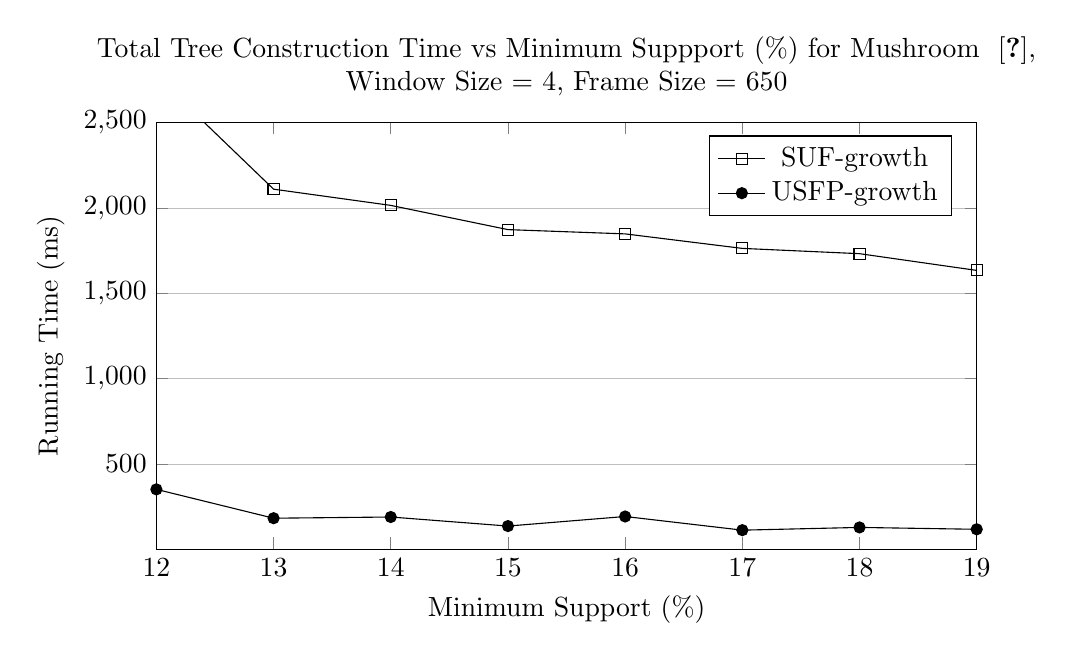
\begin{tikzpicture}
\begin{axis}[
	title={\parbox{\linewidth}{\centering Total Tree Construction Time vs Minimum Suppport (\%) for Mushroom ~\cite{dataset}, Window Size = 4, Frame Size = 650}},
	width=12cm,
	height=7cm,
    xlabel={Minimum Support (\%) },
    ylabel={Running Time (ms)},
    xmin=12, xmax=19,
    ymin=0, ymax=2500,
    xtick={12,13,14,15,16,17,18,19},
    ytick={500,1000,1500,2000,2500},
    legend pos=north east,
    ymajorgrids=true,
    grid style={line width=.2pt,draw=gray!50},
]
 
\addplot[
    solid, every mark/.append style={solid, fill=gray}, mark=square
    ]
    coordinates {
	(12,2771)
	(13,2110)
	(14,2015)
	(15,1873)
	(16,1848)
	(17,1763)
	(18,1732)
	(19,1634)
	};
    \addlegendentry{SUF-growth}
\addplot[
    solid, every mark/.append style={solid, fill=black}, mark=*
    ]
    coordinates {
	(12,351)
	(13,182)
	(14,189)
	(15,136)
	(16,192)
	(17,112)
	(18,128)
	(19,117)
};
    \addlegendentry{USFP-growth}
 
\end{axis}
\end{tikzpicture}
%\end{document}
%%mark = star, diamond, square, otimes
%\documentclass{article}
%\usepackage{pgfplots}
%\usepackage[justification=centering]{caption}
%\pgfplotsset{compat=newest}
%\begin{document}
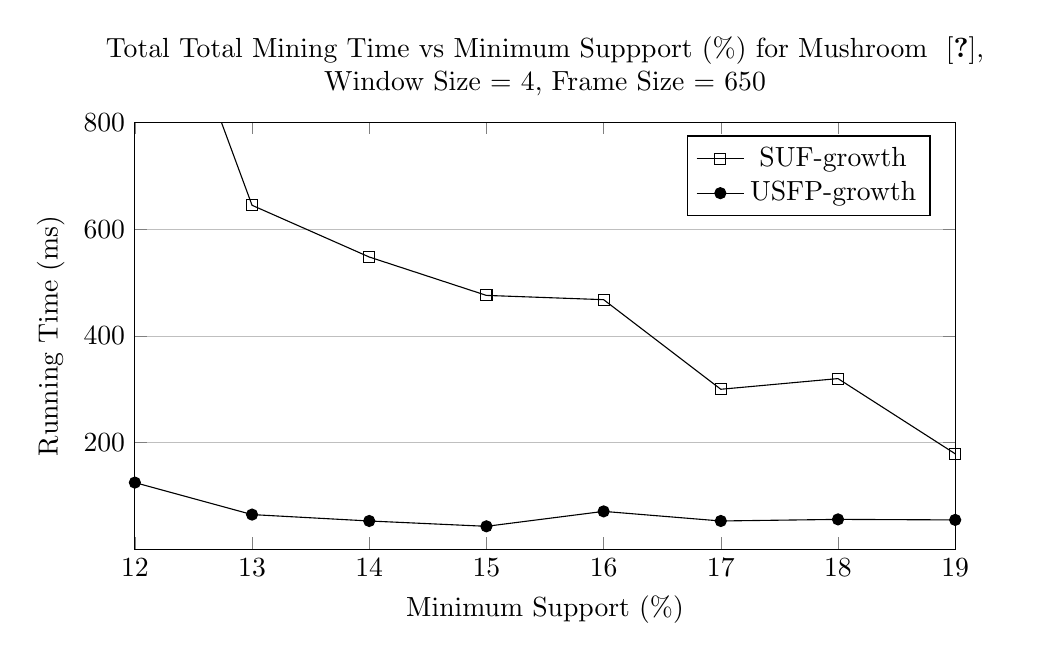
\begin{tikzpicture}
\begin{axis}[
	title={\parbox{\linewidth}{\centering Total Total Mining Time vs Minimum Suppport (\%) for Mushroom ~\cite{dataset}, Window Size = 4, Frame Size = 650}},
	width=12cm,
	height=7cm,
    xlabel={Minimum Support (\%) },
    ylabel={Running Time (ms)},
    xmin=12, xmax=19,
    ymin=0, ymax=800,
    xtick={12,13,14,15,16,17,18,19},
    ytick={200,400,600,800},
    legend pos=north east,
    ymajorgrids=true,
    grid style={line width=.2pt,draw=gray!50},
]
 
\addplot[
    solid, every mark/.append style={solid, fill=gray}, mark=square
    ]
    coordinates {
	(12,1240)
	(13,645)
	(14,548)
	(15,476)
	(16,468)
	(17,300)
	(18,320)
	(19,179)
};
    \addlegendentry{SUF-growth}
\addplot[
    solid, every mark/.append style={solid, fill=black}, mark=*
    ]
    coordinates {
	(12,125)
	(13,65 )
	(14,53 )
	(15,43 )
	(16,71 )
	(17,53 )
	(18,56 )
	(19,55 )
};
    \addlegendentry{USFP-growth}
 
\end{axis}
\end{tikzpicture}
%\end{document}
%%mark = star, diamond, square, otimes
%\documentclass{article}
%\usepackage{pgfplots}
%\usepackage[justification=centering]{caption}
%\pgfplotsset{compat=newest}
%\begin{document}
\begin{figure}[!h]
\centering

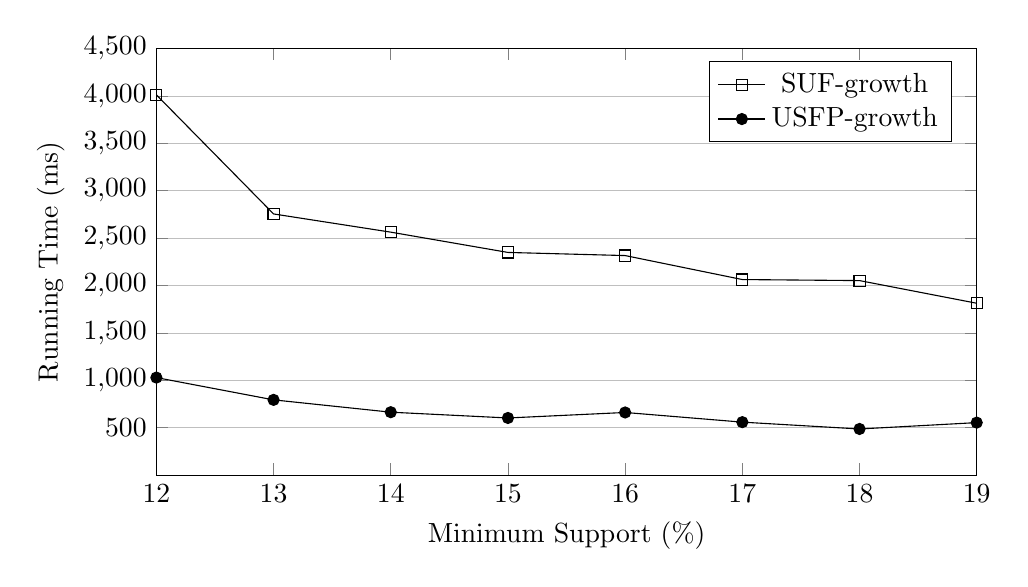
\begin{tikzpicture}
\begin{axis}[
 width=12cm,
   height=7cm,
    xlabel={Minimum Support (\%) },
    ylabel={Running Time (ms)},
    xmin=12, xmax=19,
    ymin=0, ymax=4500,
    xtick={12,13,14,15,16,17,18,19},
    ytick={500,1000,1500,2000,2500,3000,3500,4000,4500},
    legend pos=north east,
    ymajorgrids=true,
    grid style={line width=.2pt,draw=gray!50},
]
 
\addplot[
    solid, every mark/.append style={solid, fill=gray}, mark=square
    ]
    coordinates {
	(12,4011)
	(13,2755)
	(14,2563)
	(15,2349)
	(16,2316)
	(17,2063)
	(18,2052)
	(19,1813)
};
    \addlegendentry{SUF-growth}
\addplot[
    solid, every mark/.append style={solid, fill=black}, mark=*
    ]
    coordinates {
	(12,1029)
	(13,794)
	(14,664)
	(15,603)
	(16,661)
	(17,559)
	(18,487)
	(19,554)
};
    \addlegendentry{USFP-growth}
 
\end{axis}
\end{tikzpicture}
\caption{Total Time (Tree Construction + Mining + False Positive Reduction) vs Minimum Suppport (\%) \\(Window Size = 4, Frame Size = 650) for mushroom database}
\label{result:mushroom_total}
\end{figure}
%\end{document}
%%mark = star, diamond, square, otimes
%\documentclass{article}
%\usepackage{pgfplots}
%\usepackage[justification=centering]{caption}
%\pgfplotsset{compat=newest}
%\begin{document}
\begin{figure}
\centering

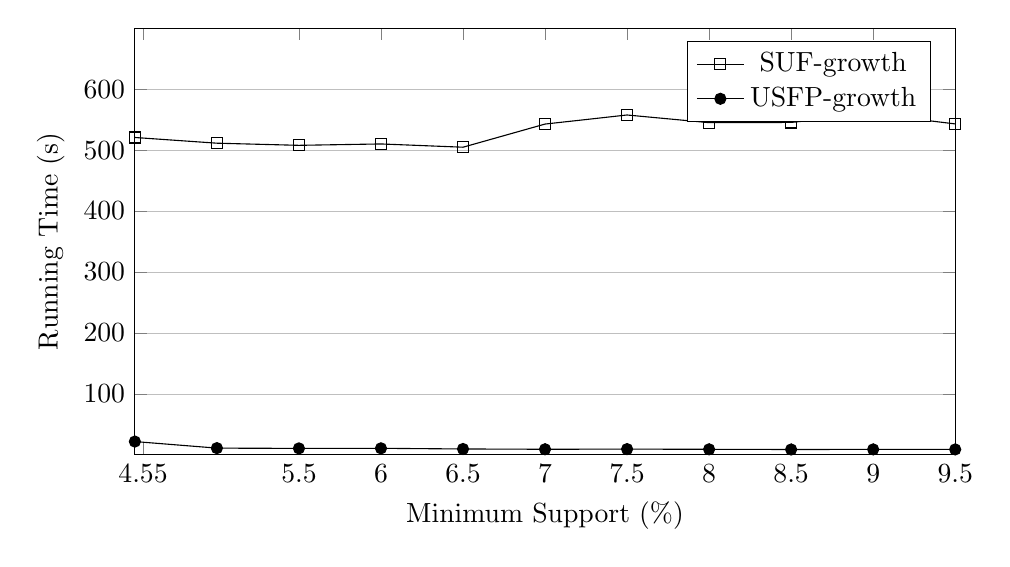
\begin{tikzpicture}
\begin{axis}[
 width=12cm,
   height=7cm,
    xlabel={Minimum Support (\%) },
    ylabel={Running Time (s)},
    xmin=4.5, xmax=9.5,
    ymin=0, ymax=700,
    xtick={4.55,5.5,6,6.5,7,7.5,8,8.5,9,9.5},
    ytick={100,200,300,400,500,600},
    legend pos=north east,
    ymajorgrids=true,
    grid style={line width=.2pt,draw=gray!50},
]
 
\addplot[
    solid, every mark/.append style={solid, fill=gray}, mark=square
    ]
    coordinates {
			(4.5,520.723)
			(5  ,511.365)
			(5.5,507.854)
			(6  ,510.12 )
			(6.5,504.767)
			(7  ,542.742)
			(7.5,557.633)
			(8  ,545.039)
			(8.5,545.444)
			(9  ,559.335)
			(9.5,542.996)

	};
    \addlegendentry{SUF-growth}
\addplot[
    solid, every mark/.append style={solid, fill=black}, mark=*
    ]
    coordinates {
		(4.5,21.814)
		(5  ,11.035)
		(5.5,10.601)
		(6  ,10.723)
		(6.5,9.646 )
		(7  ,9.177 )
		(7.5,9.427 )
		(8  ,9.092 )
		(8.5,8.8   )
		(9  ,8.95  )
		(9.5,8.883 )

};
    \addlegendentry{USFP-growth}
 
\end{axis}
\end{tikzpicture}
\caption{Total Tree Construction Time vs Minimum Suppport (\%) (Window Size = 5, Frame Size = 7000) for T40I10D100K database}
\label{result:t10_tree_total}
\end{figure}
%\end{document}
%%%mark = star, diamond, square, otimes
%\documentclass{article}
%\usepackage{pgfplots}
%\usepackage[justification=centering]{caption}
%\pgfplotsset{compat=newest}
%\begin{document}
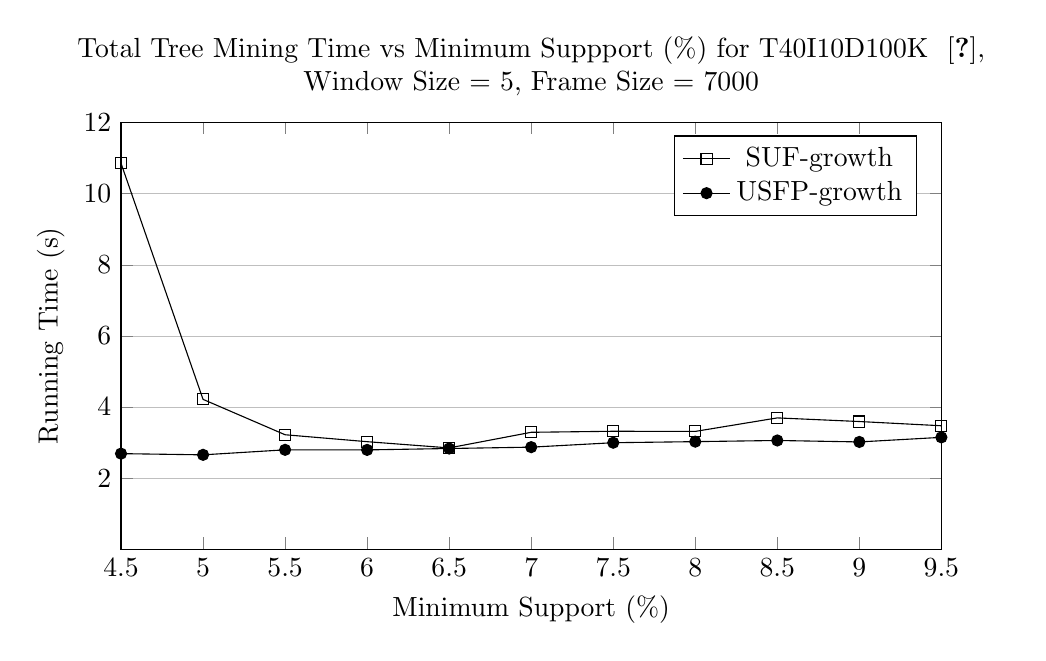
\begin{tikzpicture}
\begin{axis}[
	title={\parbox{\linewidth}{\centering Total Tree Mining Time vs Minimum Suppport (\%) for T40I10D100K ~\cite{dataset}, Window Size = 5, Frame Size = 7000}},
	width=12cm,
	height=7cm,
    xlabel={Minimum Support (\%) },
    ylabel={Running Time (s)},
    xmin=4.5, xmax=9.5,
    ymin=0, ymax=12,
    xtick={4.5,5,5.5,6,6.5,7,7.5,8,8.5,9,9.5},
    ytick={2,4,6,8,10,12},
    legend pos=north east,
    ymajorgrids=true,
    grid style={line width=.2pt,draw=gray!50},
]
 
\addplot[
    solid, every mark/.append style={solid, fill=gray}, mark=square
    ]
    coordinates {
			(4.5,10.856)
			(5  ,4.216 )
			(5.5,3.221 )
			(6  ,3.026 )
			(6.5,2.851 )
			(7  ,3.29  )
			(7.5,3.319 )
			(8  ,3.315 )
			(8.5,3.695 )
			(9  ,3.593 )
			(9.5,3.474 )

};
    \addlegendentry{SUF-growth}
\addplot[
    solid, every mark/.append style={solid, fill=black}, mark=*
    ]
    coordinates {
			(4.5,2.69  )
			(5  ,2.656 )
			(5.5,2.797 )
			(6  ,2.795 )
			(6.5,2.834 )
			(7  ,2.872 )
			(7.5,2.997 )
			(8  ,3.027 )
			(8.5,3.06  )
			(9  ,3.019 )
			(9.5,3.148 )

};
    \addlegendentry{USFP-growth}
 
\end{axis}
\end{tikzpicture}
%\end{document}
%%%mark = star, diamond, square, otimes
%\documentclass{article}
%\usepackage{pgfplots}
%\usepackage[justification=centering]{caption}
%\pgfplotsset{compat=newest}
%\begin{document}
\begin{figure}
\centering

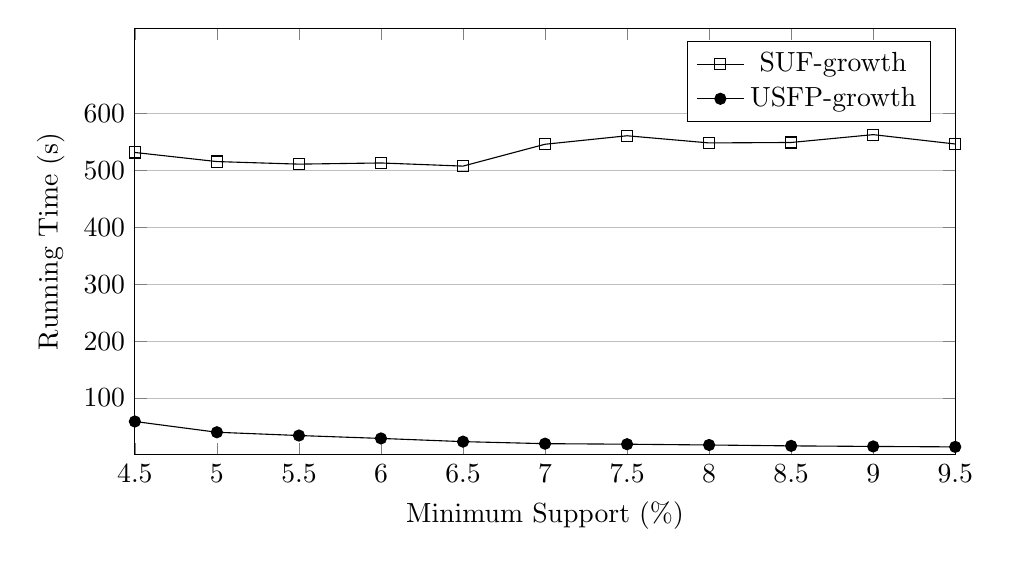
\begin{tikzpicture}
\begin{axis}[
 width=12cm,
   height=7cm,
    xlabel={Minimum Support (\%) },
    ylabel={Running Time (s)},
    xmin=4.5, xmax=9.5,
    ymin=0, ymax=750,
    xtick={4.5,5,5.5,6,6.5,7,7.5,8,8.5,9,9.5},
    ytick={100,200,300,400,500,600},
    legend pos=north east,
    ymajorgrids=true,
    grid style={line width=.2pt,draw=gray!50},
]
 
\addplot[
    solid, every mark/.append style={solid, fill=gray}, mark=square
    ]
    coordinates {
			(4.5,531.579)
			(5  ,515.581)
			(5.5,511.075)
			(6  ,513.146)
			(6.5,507.618)
			(7  ,546.032)
			(7.5,560.952)
			(8  ,548.354)
			(8.5,549.139)
			(9  ,562.928)
			(9.5,546.47 )

};
    \addlegendentry{SUF-growth}
\addplot[
    solid, every mark/.append style={solid, fill=black}, mark=*
    ]
    coordinates {
			(4.5,58.652)
			(5  ,39.735)
			(5.5,33.993)
			(6  ,28.892)
			(6.5,23.262)
			(7  ,19.669)
			(7.5,18.735)
			(8  ,17.355)
			(8.5,15.785)
			(9  ,14.803)
			(9.5,14.013)

};
    \addlegendentry{USFP-growth}
 
\end{axis}
\end{tikzpicture}
\caption{Total Time (Tree Construction + Mining + False Positive Reduction) vs Minimum Suppport (\%) (Window Size = 5, Frame Size = 7000) for T40I10D100K database}
\label{result:t10_total}
\end{figure}
%\end{document}
\cleardoublepage
\subsection{Memory Comparison}
%%mark = star, diamond, square, otimes
%\documentclass{article}
%\usepackage{pgfplots}
%\usepackage[justification=centering]{caption}
%\pgfplotsset{compat=newest}
%\begin{document}
\begin{figure}[!h]
\centering

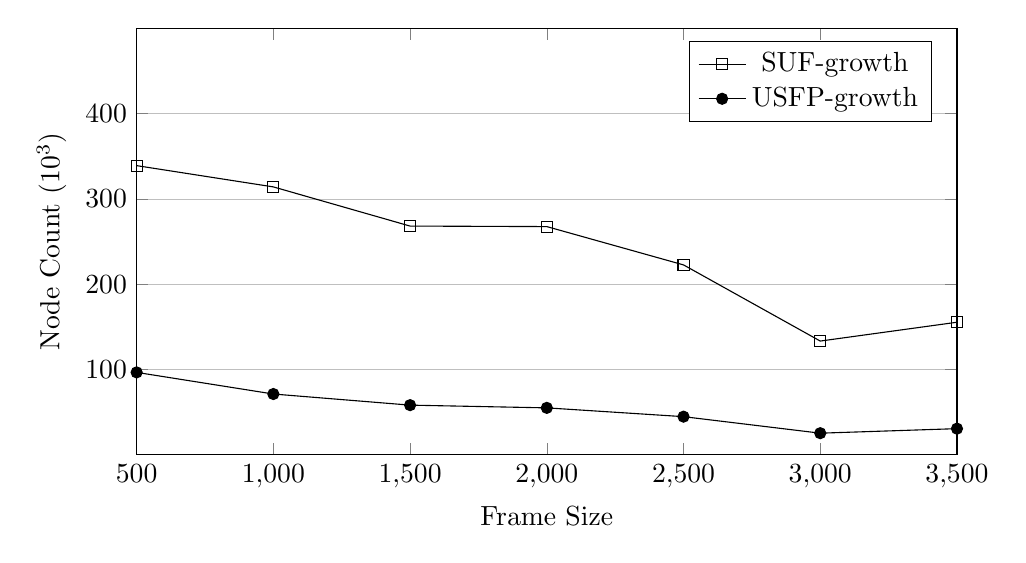
\begin{tikzpicture}
\begin{axis}[
 width=12cm,
   height=7cm,
    xlabel={Frame Size },
    ylabel={Node Count ($10^3$)},
    xmin=500, xmax=3500,
    ymin=0, ymax=500,
    xtick={500,1000,1500,2000,2500,3000,3500},
    ytick={100,200,300,400},
    legend pos=north east,
    ymajorgrids=true,
    grid style={line width=.2pt,draw=gray!50},
]
 
\addplot[
    solid, every mark/.append style={solid, fill=gray}, mark=square
    ]
    coordinates {
			(500,338.966)
			(1000,314.038)
			(1500,268.135)
			(2000,267.525)
			(2500,222.626)
			(3000,133.377)
			(3500,155.435)



	};
    \addlegendentry{SUF-growth}
\addplot[
    solid, every mark/.append style={solid, fill=black}, mark=*
    ]
    coordinates {
			(500,96.670 )
			(1000,71.314)
			(1500,58.275)
			(2000,55.086)
			(2500,44.781)
			(3000,25.416)
			(3500,30.727)


};
    \addlegendentry{USFP-growth}
 
\end{axis}
\end{tikzpicture}
\caption{Total Tree Node vs Frame Size \\(Window Size = 2) for T40I10D100K database}
\label{result:mushroom_total_mem_node}
\end{figure}
%\end{document}
%%mark = star, diamond, square, otimes
%\documentclass{article}
%\usepackage{pgfplots}
%\usepackage[justification=centering]{caption}
%\pgfplotsset{compat=newest}
%\begin{document}
\begin{figure}[!h]
\centering

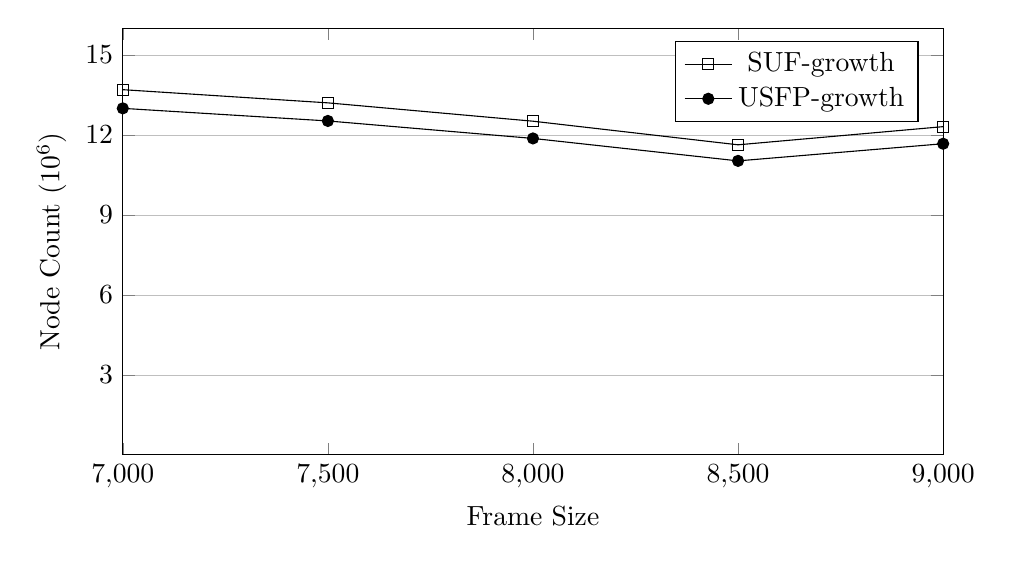
\begin{tikzpicture}
\begin{axis}[
 width=12cm,
   height=7cm,
    xlabel={Frame Size },
    ylabel={Node Count ($10^6$)},
    xmin=7000, xmax=9000,
    ymin=0, ymax=16,
    xtick={7000,7500,8000,8500,9000},
    ytick={3,6,9,12,15},
    legend pos=north east,
    ymajorgrids=true,
    grid style={line width=.2pt,draw=gray!50},
]
 
\addplot[
    solid, every mark/.append style={solid, fill=gray}, mark=square
    ]
    coordinates {
		(7000,13.695556)
		(7500,13.200902)
		(8000,12.512976)
		(8500,11.627701)
		(9000,12.308889)
		(9500,11.134408)


	};
    \addlegendentry{SUF-growth}
\addplot[
    solid, every mark/.append style={solid, fill=black}, mark=*
    ]
    coordinates {
			(7000,12.995104)
			(7500,12.522495)
			(8000,11.867025)
			(8500,11.024889)
			(9000,11.668386)
			(9500,10.552641)

};
    \addlegendentry{USFP-growth}
 
\end{axis}
\end{tikzpicture}
\caption{Total Tree Node vs Frame Size\\(Window Size = 5) for T40I10D100K database}
\label{result:t10_total_mem_node}
\end{figure}
%\end{document}
%\end{document}
%
%\end{document} % Performance Evaluation
%%%
\chapter{Conclusions}
\lhead{Chapter 5. \emph{Conclusions}}
\section{Research Summary}
In this thesis, we have proposed new window-batch based probabilistic strategy for finding frequent patterns from uncertain dynamic data. We have proposed \emph{U\textsuperscript{cap}}, which is the upper bound of existential probability. We have proposed new \emph{US-tree} data-structure that is very compact. For mining, we have proposed \emph{USFP-growth} algorithm that will efficiently and recursively mine frequent patterns from \emph{US-tree}.\\
\\
For calculating \emph{U\textsuperscript{cap}} value we have taken upper-bound of existential probability that makes the node sharing possible between same items. For uncertainty property of data node sharing was very much irregular in existing approaches. In our strategy, this sharingis allowed and that makes the tree more compact and efficient. Our proposed \emph{US-tree} is very compact for possible node sharing much more than existing tree structures (e.g. \emph{SUF-growth} ~\cite{suf_growth}). To handle the stream of data we have proposed to divide the whole transactions into batches and windows that is completely dependent on the system user how much recent data she/he wants to store in the tree. Instead of keeping the support we have kept new meta-information based on \emph{U\textsuperscript{cap}} value that helps further mining. We have developed new algorithm \emph{USFP-growth} mining algorithm that efficiently remove unnecessary patterns from the tree earlier, which helps to gain running time efficiency. Conditional candidate tree needed to be mined in our approach will be less than other approaches. This makes the mining algorithm very much faster. We have also introduced an efficient strategy to remove the false positives generated by our algorithm. Our comprehensive result study shows that total time (tree construction, tree mining, and false positive reduction) is less than existing approaches (e.g. \emph{SUF-growth} ~\cite{suf_growth}). We also developed a frequent pattern tree which may later be used to mine closed patterns and maximal patterns.
\section{Limitations and Scope of Future Studies}
As the frequent pattern mining over the domain of uncertain stream data is a very new, there are some scopes to extend and use our proposed approach as a tool for further research.\\ 
\textbf{Firstly,} we have introduced probabilistic model for calculating \emph{U\textsuperscript{cap}} value. This value can be studied and updated to find both upper and lower bound of existential probability.\\
\textbf{Secondly,} as data-set we worked on, is the stream, which is dynamic it can change dynamically. Once an item comes to the top of the \emph{US-tree} stays there at least it becomes oldest data although may be very much infrequent in the recent data. This case may make the tree not compact that was possible. As data stream cannot be read more than once. So no previously assumption can be done to this tree. So some re-construction after new batch inserted into the window will possibly be the one of the major optimization of the tree.
\section{Conclusions}
 % Conclusion



\addtocontents{toc}{\vspace{2em}}  % Add a gap in the Contents, for aesthetics
\backmatter

%% ----------------------------------------------------------------
\label{Bibliography}
\lhead{\emph{Bibliography}}  % Change the left side page header to "Bibliography"
%\bibliographystyle{unsrtnat}  % Use the "unsrtnat" BibTeX style for formatting the Bibliography
\bibliographystyle{plain}
%\bibliography{mybib}
\bibliography{Bibliography}   % The references (bibliography) information are stored in the file named "Bibliography.bib"

\clearpage
~\cite{uh_mining}
~\cite{puf_growth}
~\cite{cuf_growth}
~\cite{ufp_growth}
~\cite{uf_growth}
~\cite{u_priori}
~\cite{const_01}
~\cite{apriori}
~\cite{fp_growth}
~\cite{ass_01}
~\cite{gsp}
~\cite{prefix_span}
~\cite{ds_tree}
~\cite{rps_tree}
~\cite{hup_mining}
~\cite{g_span}
~\cite{close_1}
~\cite{closet}
~\cite{closet_plus}
~\cite{tpf}
~\cite{close_2}
~\cite{charm}
~\cite{ass_02}
~\cite{ass_03}
~\cite{ass_04}
~\cite{ass_05}
~\cite{ass_06}
~\cite{ass_07}
~\cite{sqn_02}
~\cite{sqn_02}
~\cite{sqn_02}
~\cite{suf_growth}
~\cite{stream_01}
~\cite{stream_02}
~\cite{stream_03}
~\cite{stream_05}
~\cite{uncertain_01}
~\cite{uncertain_02}
~\cite{uncertain_03}
~\cite{uncertain_04}
~\cite{uncertain_05}
~\cite{uncertain_06}
~\cite{facebook}
~\cite{twitter}
\end{document}  % The End
%% ----------------------------------------------------------------